\documentclass{article}
\usepackage{latexsym,amsmath,xcolor,multicol,booktabs,calligra,subfigure}
\usepackage{ctex,hyperref,graphicx,pstricks,listings,stackengine,tikz,listings}
\usetikzlibrary{angles}
\usetikzlibrary{quotes,patterns,decorations.pathreplacing}
\graphicspath{{pic/}}
\definecolor{primaryD}{HTML}{00695C}
\lstset{
	language=[ISO]C++,
	%basicstyle=\ttfamily\footnotesize,
	basicstyle=\ttfamily\small, 
	tabsize=2,
	keywordstyle=\bfseries\ttfamily\color{primaryD},
	commentstyle=\sl\ttfamily\color[RGB]{100,100,100},
	stringstyle=\ttfamily\color[RGB]{50,50,50},
	extendedchars=true,
	breaklines=true,
	numbers=left, 
	frame=shadowbox, 
	rulesepcolor=\color{red!20!green!20!blue!20},
}
\begin{document}


\begin{tikzpicture}[scale=0.1]
\draw[color=violet](28,-4)--(28,-0);
\draw[color=violet](28,-8)--(28,-5)--(27,-5)--(27,-0);
\draw[color=violet](28,-12)--(28,-9)--(29,-9)--(29,-0);
\draw[color=violet](28,-16)--(28,-13)--(27,-13)--(27,-6)--(26,-6)--(26,-0);
\draw[color=violet](28,-20)--(28,-17)--(29,-17)--(29,-10)--(30,-10)--(30,-0);
\draw[color=violet](28,-24)--(28,-21)--(27,-21)--(27,-14)--(26,-14)--(26,-7)--(25,-7)--(25,-0);
%\draw[color=violet](28,-28)--(28,-31)--(29,-31)--(29,-38)--(30,-38)--(30,-45)--(31,-45)--(31,-52);
\draw[color=violet](28,-32)--(28,-35)--(27,-35)--(27,-42)--(26,-42)--(26,-52);
\draw[color=violet](28,-36)--(28,-39)--(29,-39)--(29,-46)--(30,-46)--(30,-52);
\draw[color=violet](28,-40)--(28,-43)--(27,-43)--(27,-52);
\draw[color=violet](28,-44)--(28,-47)--(29,-47)--(29,-52);
\draw[color=violet](28,-48)--(28,-52);
\end{tikzpicture}

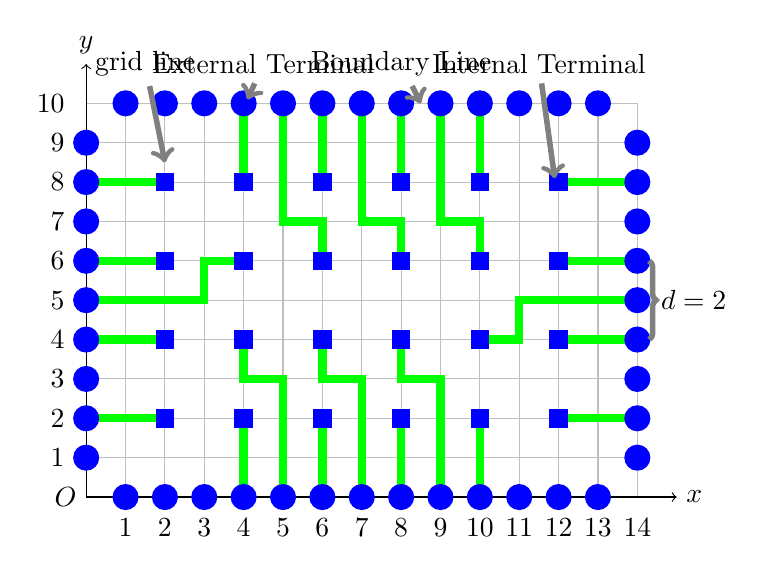
\begin{tikzpicture}[decoration=brace,scale=0.5]
\foreach \x in {0,1,...,14}
\draw[color=lightgray](\x,0)--(\x,10);
\foreach \x in {0,1,...,10}
\draw[color=lightgray](0,\x)--(14,\x);
\draw[->] (0,0) -- (15,0) node[right] {$x$};
\draw[->] (0,0) -- (0,11) node[above] {$y$};
\node[below,left]at(0,0){$O$};
\foreach \x in {1,2,...,14}
\node[below]at(\x,-0.3){$\x$};
\foreach \x in {1,2,...,10}
\node[left]at(-0.3,\x){$\x$};
\draw[color=green,line width=3pt](2,2)--(0,2);
\draw[color=green,line width=3pt](2,4)--(0,4);
\draw[color=green,line width=3pt](2,6)--(0,6);
\draw[color=green,line width=3pt](2,8)--(0,8);
\draw[color=green,line width=3pt](4,2)--(4,0);
\draw[color=green,line width=3pt](4,4)--(4,3)--(5,3)--(5,0);
\draw[color=green,line width=3pt](4,6)--(3,6)--(3,5)--(0,5);
\draw[color=green,line width=3pt](4,8)--(4,10);
\draw[color=green,line width=3pt](6,2)--(6,0);
\draw[color=green,line width=3pt](6,4)--(6,3)--(7,3)--(7,0);
\draw[color=green,line width=3pt](6,6)--(6,7)--(5,7)--(5,10);
\draw[color=green,line width=3pt](6,8)--(6,10);
\draw[color=green,line width=3pt](8,2)--(8,0);
\draw[color=green,line width=3pt](8,4)--(8,3)--(9,3)--(9,0);
\draw[color=green,line width=3pt](8,6)--(8,7)--(7,7)--(7,10);
\draw[color=green,line width=3pt](8,8)--(8,10);
\draw[color=green,line width=3pt](10,2)--(10,0);
\draw[color=green,line width=3pt](10,4)--(11,4)--(11,5)--(14,5);
\draw[color=green,line width=3pt](10,6)--(10,7)--(9,7)--(9,10);
\draw[color=green,line width=3pt](10,8)--(10,10);
\draw[color=green,line width=3pt](12,2)--(14,2);
\draw[color=green,line width=3pt](12,4)--(14,4);
\draw[color=green,line width=3pt](12,6)--(14,6);
\draw[color=green,line width=3pt](12,8)--(14,8);
\foreach \x in {1,2,...,13}{
	\node[shape=circle,fill=blue]at(\x,0){};
	\node[shape=circle,fill=blue]at(\x,10){};
}
\foreach \x in {1,2,...,9}{
	\node[shape=circle,fill=blue]at(0,\x){};
	\node[shape=circle,fill=blue]at(14,\x){};
}
\foreach \x in {2,4,...,12}
\foreach \y in {2,4,6,8}
\node[shape=rectangle,fill=blue]at(\x,\y){};
\node(gl)at (1.5,11){grid line};
\draw[->,line width=2pt,color=gray](gl)--(2,8.5);
\node(et)at(4.5,11){External Terminal};
\draw[->,line width=2pt,color=gray](et)--(4.1,10.1);
\node(bl)at(8,11){Boundary Line};
\draw[->,line width=2pt,color=gray](bl)--(8.5,10);
\node(it)at(11.5,11){Internal Terminal};
\draw[->,line width=2pt,color=gray](it)--(11.9,8.1);

\draw [decorate,line width=2pt,color=gray] (14.3,6) --node [right,color=black]{$d=2$} (14.3,4);

\end{tikzpicture}

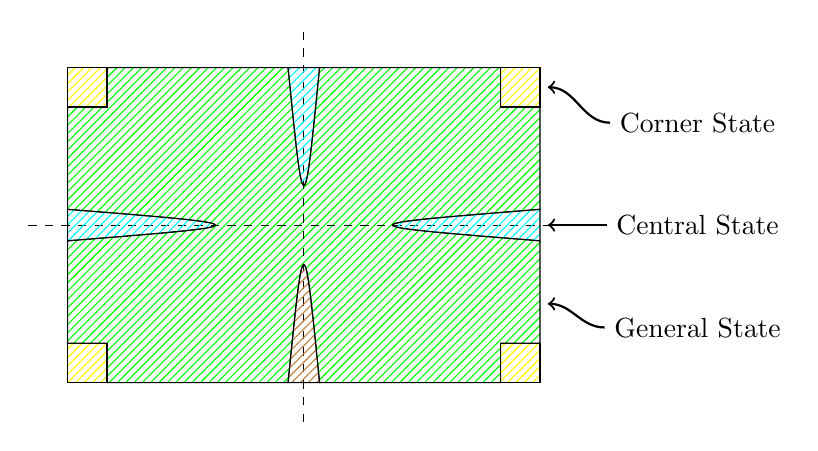
\begin{tikzpicture}
	\draw[pattern color=green, pattern=north east lines](0,0.5)--(0.5,0.5)--(0.5,0)--(2.8,0) .. controls (3,2) .. (3.2,0)--(5.5,0)--(5.5,0.5)--(6,0.5)--(6,1.8) .. controls (3.5,2) .. (6,2.2)--(6,3.5)--(5.5,3.5)--(5.5,4)--(3.2,4) .. controls (3,2) .. (2.8,4)--(0.5,4)--(0.5,3.5)--(0,3.5)--(0,2.2) .. controls (2.5,2) .. (0,1.8)--cycle;
	\draw[dashed](3,-0.5)--(3,4.5);
	\draw[dashed](-0.5,2)--(6.5,2);
	\draw[pattern color=brown, pattern=north east lines](2.8,0) .. controls (3,2) .. (3.2,0)--cycle;
	\draw[pattern color=cyan, pattern=north east lines](2.8,4) .. controls (3,2) .. (3.2,4)--cycle;
	\draw[pattern color=cyan, pattern=north east lines](0,1.8) .. controls (2.5,2) .. (0,2.2)--cycle;
	\draw[pattern color=cyan, pattern=north east lines](6,1.8) .. controls (3.5,2) .. (6,2.2)--cycle;
	\draw[pattern color=yellow, pattern=north east lines](0.5,0)--(0.5,0.5)--(0,0.5)--(0,0)--cycle;
	\draw[pattern color=yellow, pattern=north east lines](0.5,4)--(0.5,3.5)--(0,3.5)--(0,4)--cycle;
	\draw[pattern color=yellow, pattern=north east lines](5.5,4)--(5.5,3.5)--(6,3.5)--(6,4)--cycle;
	\draw[pattern color=yellow, pattern=north east lines](5.5,0)--(5.5,0.5)--(6,0.5)--(6,0)--cycle;
	\node (corner) at (8,3.3) {Corner State};
	\draw [->,thick] (corner) to [in = 0, out = 180] (6.1,3.75);
	\node (central) at (8,2) {Central State};
	\draw [->,thick] (central) to [in = 0, out = 180] (6.1,2);
	\node (general) at (8,0.7) {General State};
	\draw [->,thick] (general) to [in = 0, out = 180] (6.1,1);
	
\end{tikzpicture}

\begin{figure}
\begin{center}
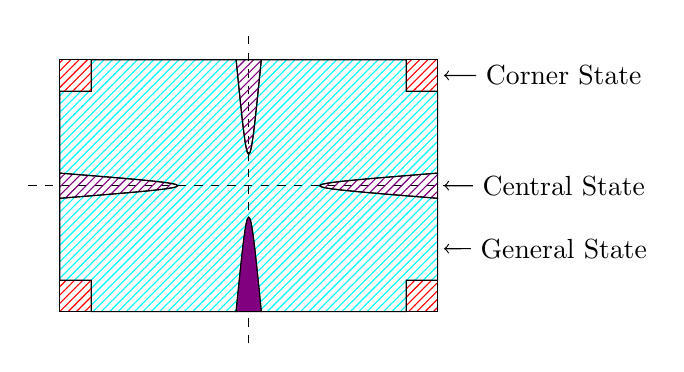
\begin{tikzpicture}[scale=0.8]
	\draw[pattern color=cyan, pattern=north east lines](0,0.5)--(0.5,0.5)--(0.5,0)--(2.8,0) .. controls (3,2) .. (3.2,0)--(5.5,0)--(5.5,0.5)--(6,0.5)--(6,1.8) .. controls (3.5,2) .. (6,2.2)--(6,3.5)--(5.5,3.5)--(5.5,4)--(3.2,4) .. controls (3,2) .. (2.8,4)--(0.5,4)--(0.5,3.5)--(0,3.5)--(0,2.2) .. controls (2.5,2) .. (0,1.8)--cycle;
	\draw[dashed](3,-0.5)--(3,4.5);
	\draw[dashed](-0.5,2)--(6.5,2);
	\draw[fill=violet](2.8,0) .. controls (3,2) .. (3.2,0)--cycle;
	\draw[pattern color=violet, pattern=north east lines](2.8,4) .. controls (3,2) .. (3.2,4)--cycle;
	\draw[pattern color=violet, pattern=north east lines](0,1.8) .. controls (2.5,2) .. (0,2.2)--cycle;
	\draw[pattern color=violet, pattern=north east lines](6,1.8) .. controls (3.5,2) .. (6,2.2)--cycle;
	\draw[pattern color=red, pattern=north east lines](0.5,0)--(0.5,0.5)--(0,0.5)--(0,0)--cycle;
	\draw[pattern color=red, pattern=north east lines](0.5,4)--(0.5,3.5)--(0,3.5)--(0,4)--cycle;
	\draw[pattern color=red, pattern=north east lines](5.5,4)--(5.5,3.5)--(6,3.5)--(6,4)--cycle;
	\draw[pattern color=red, pattern=north east lines](5.5,0)--(5.5,0.5)--(6,0.5)--(6,0)--cycle;
	\node (corner) at (8,3.75) {Corner State};
	\draw [->] (corner) -- (6.1,3.75);
	\node (central) at (8,2) {Central State};
	\draw [->] (central) -- (6.1,2);
	\node (general) at (8,1) {General State};
	\draw [->] (general) -- (6.1,1);
\end{tikzpicture}
\caption{Example of Routing States}
\label{img:state}
\end{center}
\end{figure}


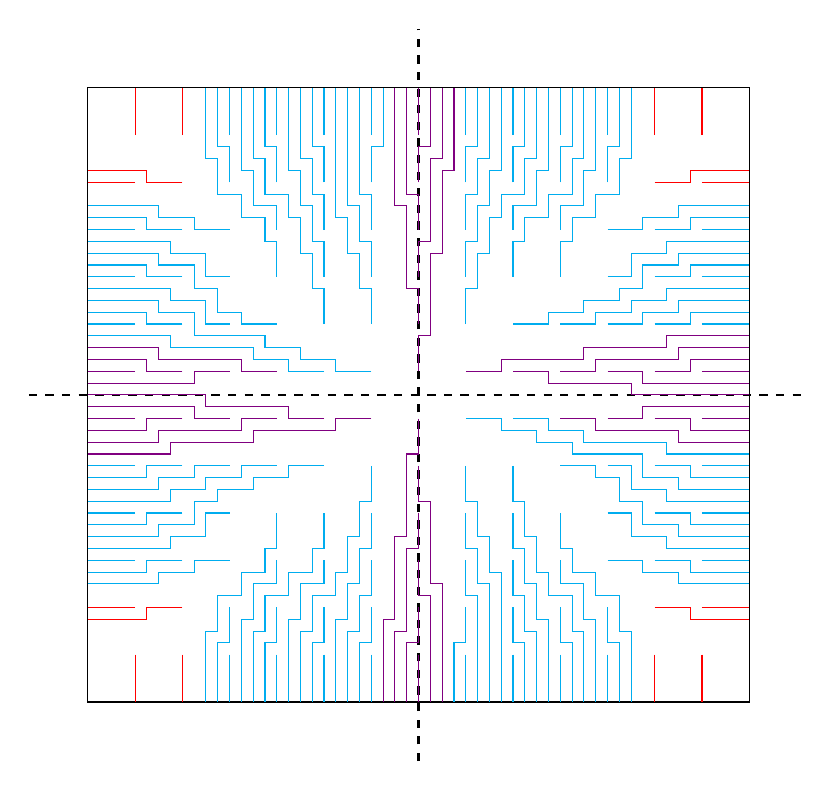
\begin{tikzpicture}[scale=0.15]
\draw(0,0)--(0,52)--(56,52)--(56,0)--cycle;
\draw[dashed,thick](-5,26)--(61,26);
\draw[dashed,thick](28,-5)--(28,57);
\draw[color=red](4,4)--(4,0);
\draw[color=red](4,8)--(0,8);
\draw[color=cyan](4,12)--(0,12);
\draw[color=cyan](4,16)--(0,16);
\draw[color=cyan](4,20)--(0,20);
\draw[color=violet](4,24)--(0,24);
\draw[color=violet](4,28)--(0,28);
\draw[color=cyan](4,32)--(0,32);
\draw[color=cyan](4,36)--(0,36);
\draw[color=cyan](4,40)--(0,40);
\draw[color=red](4,44)--(0,44);
\draw[color=red](4,48)--(4,52);
\draw[color=red](8,4)--(8,0);
\draw[color=red](8,8)--(5,8)--(5,7)--(0,7);
\draw[color=cyan](8,12)--(5,12)--(5,11)--(0,11);
\draw[color=cyan](8,16)--(5,16)--(5,15)--(0,15);
\draw[color=cyan](8,20)--(5,20)--(5,19)--(0,19);
\draw[color=violet](8,24)--(5,24)--(5,23)--(0,23);
\draw[color=violet](8,28)--(5,28)--(5,29)--(0,29);
\draw[color=cyan](8,32)--(5,32)--(5,33)--(0,33);
\draw[color=cyan](8,36)--(5,36)--(5,37)--(0,37);
\draw[color=cyan](8,40)--(5,40)--(5,41)--(0,41);
\draw[color=red](8,44)--(5,44)--(5,45)--(0,45);
\draw[color=red](8,48)--(8,52);
\draw[color=cyan](12,4)--(12,0);
\draw[color=cyan](12,8)--(12,5)--(11,5)--(11,0);
\draw[color=cyan](12,12)--(9,12)--(9,11)--(6,11)--(6,10)--(0,10);
\draw[color=cyan](12,16)--(10,16)--(10,14)--(7,14)--(7,13)--(0,13);
\draw[color=cyan](12,20)--(9,20)--(9,19)--(6,19)--(6,18)--(0,18);
\draw[color=violet](12,24)--(9,24)--(9,25)--(0,25);
\draw[color=violet](12,28)--(9,28)--(9,27)--(0,27);
\draw[color=cyan](12,32)--(10,32)--(10,34)--(7,34)--(7,35)--(0,35);
\draw[color=cyan](12,36)--(10,36)--(10,38)--(7,38)--(7,39)--(0,39);
\draw[color=cyan](12,40)--(9,40)--(9,41)--(6,41)--(6,42)--(0,42);
\draw[color=cyan](12,44)--(12,47)--(11,47)--(11,52);
\draw[color=cyan](12,48)--(12,52);
\draw[color=cyan](16,4)--(16,0);
\draw[color=cyan](16,8)--(16,5)--(15,5)--(15,0);
\draw[color=cyan](16,12)--(16,10)--(14,10)--(14,7)--(13,7)--(13,0);
\draw[color=cyan](16,16)--(16,13)--(15,13)--(15,11)--(13,11)--(13,9)--(11,9)--(11,6)--(10,6)--(10,0);
\draw[color=cyan](16,20)--(13,20)--(13,19)--(10,19)--(10,18)--(7,18)--(7,17)--(0,17);
\draw[color=violet](16,24)--(13,24)--(13,23)--(6,23)--(6,22)--(0,22);
\draw[color=violet](16,28)--(13,28)--(13,29)--(6,29)--(6,30)--(0,30);
\draw[color=cyan](16,32)--(13,32)--(13,33)--(11,33)--(11,35)--(9,35)--(9,37)--(6,37)--(6,38)--(0,38);
\draw[color=cyan](16,36)--(16,39)--(15,39)--(15,41)--(13,41)--(13,43)--(11,43)--(11,46)--(10,46)--(10,52);
\draw[color=cyan](16,40)--(16,42)--(14,42)--(14,45)--(13,45)--(13,52);
\draw[color=cyan](16,44)--(16,47)--(15,47)--(15,52);
\draw[color=cyan](16,48)--(16,52);
\draw[color=cyan](20,4)--(20,0);
\draw[color=cyan](20,8)--(20,5)--(19,5)--(19,0);
\draw[color=cyan](20,12)--(20,10)--(18,10)--(18,7)--(17,7)--(17,0);
\draw[color=cyan](20,16)--(20,13)--(19,13)--(19,11)--(17,11)--(17,9)--(15,9)--(15,6)--(14,6)--(14,0);
\draw[color=cyan](20,20)--(17,20)--(17,19)--(14,19)--(14,18)--(11,18)--(11,17)--(9,17)--(9,15)--(6,15)--(6,14)--(0,14);
\draw[color=violet](20,24)--(17,24)--(17,25)--(10,25)--(10,26)--(0,26);
\draw[color=cyan](20,28)--(17,28)--(17,29)--(14,29)--(14,30)--(7,30)--(7,31)--(0,31);
\draw[color=cyan](20,32)--(20,35)--(19,35)--(19,38)--(18,38)--(18,41)--(17,41)--(17,43)--(15,43)--(15,46)--(14,46)--(14,52);
\draw[color=cyan](20,36)--(20,39)--(19,39)--(19,42)--(18,42)--(18,45)--(17,45)--(17,52);
\draw[color=cyan](20,40)--(20,43)--(19,43)--(19,46)--(18,46)--(18,52);
\draw[color=cyan](20,44)--(20,47)--(19,47)--(19,52);
\draw[color=cyan](20,48)--(20,52);
\draw[color=cyan](24,4)--(24,0);
\draw[color=cyan](24,8)--(24,5)--(23,5)--(23,0);
\draw[color=cyan](24,12)--(24,9)--(23,9)--(23,6)--(22,6)--(22,0);
\draw[color=cyan](24,16)--(24,13)--(23,13)--(23,10)--(22,10)--(22,7)--(21,7)--(21,0);
\draw[color=cyan](24,20)--(24,17)--(23,17)--(23,14)--(22,14)--(22,11)--(21,11)--(21,9)--(19,9)--(19,6)--(18,6)--(18,0);
\draw[color=violet](24,24)--(21,24)--(21,23)--(14,23)--(14,22)--(7,22)--(7,21)--(0,21);
\draw[color=cyan](24,28)--(21,28)--(21,29)--(18,29)--(18,30)--(15,30)--(15,31)--(9,31)--(9,33)--(6,33)--(6,34)--(0,34);
\draw[color=cyan](24,32)--(24,35)--(23,35)--(23,38)--(22,38)--(22,41)--(21,41)--(21,52);
\draw[color=cyan](24,36)--(24,39)--(23,39)--(23,42)--(22,42)--(22,52);
\draw[color=cyan](24,40)--(24,43)--(23,43)--(23,52);
\draw[color=cyan](24,44)--(24,47)--(25,47)--(25,52);
\draw[color=cyan](24,48)--(24,52);
\draw[color=violet](28,4)--(28,0);
\draw[color=violet](28,8)--(28,5)--(27,5)--(27,0);
\draw[color=violet](28,12)--(28,9)--(29,9)--(29,0);
\draw[color=violet](28,16)--(28,13)--(27,13)--(27,6)--(26,6)--(26,0);
\draw[color=violet](28,20)--(28,17)--(29,17)--(29,10)--(30,10)--(30,0);
\draw[color=violet](28,24)--(28,21)--(27,21)--(27,14)--(26,14)--(26,7)--(25,7)--(25,0);
\draw[color=violet](28,28)--(28,31)--(29,31)--(29,38)--(30,38)--(30,45)--(31,45)--(31,52);
\draw[color=violet](28,32)--(28,35)--(27,35)--(27,42)--(26,42)--(26,52);
\draw[color=violet](28,36)--(28,39)--(29,39)--(29,46)--(30,46)--(30,52);
\draw[color=violet](28,40)--(28,43)--(27,43)--(27,52);
\draw[color=violet](28,44)--(28,47)--(29,47)--(29,52);
\draw[color=violet](28,48)--(28,52);
\draw[color=cyan](32,4)--(32,0);
\draw[color=cyan](32,8)--(32,5)--(31,5)--(31,0);
\draw[color=cyan](32,12)--(32,9)--(33,9)--(33,0);
\draw[color=cyan](32,16)--(32,13)--(33,13)--(33,10)--(34,10)--(34,0);
\draw[color=cyan](32,20)--(32,17)--(33,17)--(33,14)--(34,14)--(34,11)--(35,11)--(35,0);
\draw[color=cyan](32,24)--(35,24)--(35,23)--(38,23)--(38,22)--(41,22)--(41,21)--(47,21)--(47,19)--(50,19)--(50,18)--(56,18);
\draw[color=violet](32,28)--(35,28)--(35,29)--(42,29)--(42,30)--(49,30)--(49,31)--(56,31);
\draw[color=cyan](32,32)--(32,35)--(33,35)--(33,38)--(34,38)--(34,41)--(35,41)--(35,43)--(37,43)--(37,46)--(38,46)--(38,52);
\draw[color=cyan](32,36)--(32,39)--(33,39)--(33,42)--(34,42)--(34,45)--(35,45)--(35,52);
\draw[color=cyan](32,40)--(32,43)--(33,43)--(33,46)--(34,46)--(34,52);
\draw[color=cyan](32,44)--(32,47)--(33,47)--(33,52);
\draw[color=cyan](32,48)--(32,52);
\draw[color=cyan](36,4)--(36,0);
\draw[color=cyan](36,8)--(36,5)--(37,5)--(37,0);
\draw[color=cyan](36,12)--(36,9)--(37,9)--(37,6)--(38,6)--(38,0);
\draw[color=cyan](36,16)--(36,13)--(37,13)--(37,10)--(38,10)--(38,7)--(39,7)--(39,0);
\draw[color=cyan](36,20)--(36,17)--(37,17)--(37,14)--(38,14)--(38,11)--(39,11)--(39,9)--(41,9)--(41,6)--(42,6)--(42,0);
\draw[color=cyan](36,24)--(39,24)--(39,23)--(42,23)--(42,22)--(49,22)--(49,21)--(56,21);
\draw[color=violet](36,28)--(39,28)--(39,27)--(46,27)--(46,26)--(56,26);
\draw[color=cyan](36,32)--(39,32)--(39,33)--(42,33)--(42,34)--(45,34)--(45,35)--(47,35)--(47,37)--(50,37)--(50,38)--(56,38);
\draw[color=cyan](36,36)--(36,39)--(37,39)--(37,41)--(39,41)--(39,43)--(41,43)--(41,46)--(42,46)--(42,52);
\draw[color=cyan](36,40)--(36,42)--(38,42)--(38,45)--(39,45)--(39,52);
\draw[color=cyan](36,44)--(36,47)--(37,47)--(37,52);
\draw[color=cyan](36,48)--(36,52);
\draw[color=cyan](40,4)--(40,0);
\draw[color=cyan](40,8)--(40,5)--(41,5)--(41,0);
\draw[color=cyan](40,12)--(40,10)--(42,10)--(42,7)--(43,7)--(43,0);
\draw[color=cyan](40,16)--(40,13)--(41,13)--(41,11)--(43,11)--(43,9)--(45,9)--(45,6)--(46,6)--(46,0);
\draw[color=cyan](40,20)--(43,20)--(43,19)--(45,19)--(45,17)--(47,17)--(47,15)--(50,15)--(50,14)--(56,14);
\draw[color=violet](40,24)--(43,24)--(43,23)--(50,23)--(50,22)--(56,22);
\draw[color=violet](40,28)--(43,28)--(43,29)--(50,29)--(50,30)--(56,30);
\draw[color=cyan](40,32)--(43,32)--(43,33)--(46,33)--(46,34)--(49,34)--(49,35)--(56,35);
\draw[color=cyan](40,36)--(40,39)--(41,39)--(41,41)--(43,41)--(43,43)--(45,43)--(45,46)--(46,46)--(46,52);
\draw[color=cyan](40,40)--(40,42)--(42,42)--(42,45)--(43,45)--(43,52);
\draw[color=cyan](40,44)--(40,47)--(41,47)--(41,52);
\draw[color=cyan](40,48)--(40,52);
\draw[color=cyan](44,4)--(44,0);
\draw[color=cyan](44,8)--(44,5)--(45,5)--(45,0);
\draw[color=cyan](44,12)--(47,12)--(47,11)--(50,11)--(50,10)--(56,10);
\draw[color=cyan](44,16)--(46,16)--(46,14)--(49,14)--(49,13)--(56,13);
\draw[color=cyan](44,20)--(46,20)--(46,18)--(49,18)--(49,17)--(56,17);
\draw[color=violet](44,24)--(47,24)--(47,25)--(56,25);
\draw[color=violet](44,28)--(47,28)--(47,27)--(56,27);
\draw[color=cyan](44,32)--(47,32)--(47,33)--(50,33)--(50,34)--(56,34);
\draw[color=cyan](44,36)--(46,36)--(46,38)--(49,38)--(49,39)--(56,39);
\draw[color=cyan](44,40)--(47,40)--(47,41)--(50,41)--(50,42)--(56,42);
\draw[color=cyan](44,44)--(44,47)--(45,47)--(45,52);
\draw[color=cyan](44,48)--(44,52);
\draw[color=red](48,4)--(48,0);
\draw[color=red](48,8)--(51,8)--(51,7)--(56,7);
\draw[color=cyan](48,12)--(51,12)--(51,11)--(56,11);
\draw[color=cyan](48,16)--(51,16)--(51,15)--(56,15);
\draw[color=cyan](48,20)--(51,20)--(51,19)--(56,19);
\draw[color=violet](48,24)--(51,24)--(51,23)--(56,23);
\draw[color=violet](48,28)--(51,28)--(51,29)--(56,29);
\draw[color=cyan](48,32)--(51,32)--(51,33)--(56,33);
\draw[color=cyan](48,36)--(51,36)--(51,37)--(56,37);
\draw[color=cyan](48,40)--(51,40)--(51,41)--(56,41);
\draw[color=red](48,44)--(51,44)--(51,45)--(56,45);
\draw[color=red](48,48)--(48,52);
\draw[color=red](52,4)--(52,0);
\draw[color=red](52,8)--(56,8);
\draw[color=cyan](52,12)--(56,12);
\draw[color=cyan](52,16)--(56,16);
\draw[color=cyan](52,20)--(56,20);
\draw[color=violet](52,24)--(56,24);
\draw[color=violet](52,28)--(56,28);
\draw[color=cyan](52,32)--(56,32);
\draw[color=cyan](52,36)--(56,36);
\draw[color=cyan](52,40)--(56,40);
\draw[color=red](52,44)--(56,44);
\draw[color=red](52,48)--(52,52);
\end{tikzpicture}

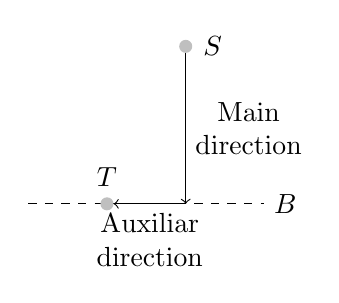
\begin{tikzpicture}
\draw[dashed](1,0)--(4,0)node[right]{$B$};
\node[fill=lightgray,shape=circle,scale=0.5](s) at (3,2){};
\node[fill=lightgray,shape=circle,scale=0.5](t) at (2,0){};
\node[right] at (3.1,2){$S$};
\node[above] at (2,0.1){$T$};
\draw[->](s)--node[align=center,right]{Main\\direction}(3,0);
\draw[->](3,0)--node[align=center,below]{Auxiliar\\direction}(t);
\end{tikzpicture}

\begin{figure}[htbp]
%%\vspace{-0.45cm}
\centering
\subfigure[]
{
\begin{minipage}[b]{0.9\columnwidth}
\centering
\resizebox{\columnwidth}{!}{
}
\label{fig:region:a}
\end{minipage}%
}%
\hfil
%%\vspace{-0.25cm}
\subfigure[]
{
\begin{minipage}[b]{0.9\columnwidth}
\centering
\resizebox{\columnwidth}{!}{
}
\label{fig:region:b}
\end{minipage}%
}%
%\vspace{-0.2cm}
%\vspace{-0.25cm}
\end{figure}

\begin{figure}[htbp]
%%\vspace{-0.45cm}
\centering
\subfigure[]
{
\label{fig:rule1:a}
\begin{minipage}[b]{0.48\columnwidth}
\centering
\resizebox{\columnwidth}{!}{
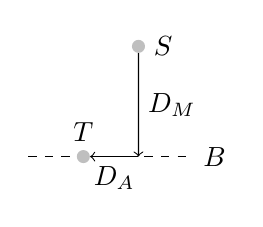
\begin{tikzpicture}[scale=0.7]
\draw[dashed](1,0)--(4,0)node[right]{$B$};
\node[fill=lightgray,shape=circle,scale=0.5](s) at (3,2){};
\node[fill=lightgray,shape=circle,scale=0.5](t) at (2,0){};
\node[right] at (3.1,2){$S$};
\node[above] at (2,0.1){$T$};
\draw[->](s)--node[align=center,right]{$D_M$}(3,0);
\draw[->](3,0)--node[align=center,below]{$D_A$}(t);
\end{tikzpicture}
}
\end{minipage}%
}%
\hfil
%%\vspace{-0.25cm}
\subfigure[]
{
\label{fig:rule1:b}
\begin{minipage}[b]{0.48\columnwidth}
\centering
\resizebox{\columnwidth}{!}{

\begin{tikzpicture}[scale=0.05]
\draw[color=violet](28,-32)--(28,-35)--(27,-35)--(27,-42)--(26,-42)--(26,-52);
\draw[color=violet](28,-36)--(28,-39)--(29,-39)--(29,-46)--(30,-46)--(30,-52);
\draw[color=violet](28,-40)--(28,-43)--(27,-43)--(27,-52);
\draw[color=violet](28,-44)--(28,-47)--(29,-47)--(29,-52);
\draw[color=violet](28,-48)--(28,-52);
\end{tikzpicture}
}
\end{minipage}%
}%
%%\vspace{-0.2cm}
\caption{(a)Main direction and Auxiliar direction; (b)  }
\label{fig:rule1}
%%\vspace{-0.25cm}
\end{figure}



\end{document}